% LuaLaTeX

\documentclass[a4paper, twoside, 12pt]{article}
\usepackage[latin]{babel}
%\usepackage[landscape, left=3cm, right=1.5cm, top=2cm, bottom=1cm]{geometry} % okraje stranky
%\usepackage[landscape, a4paper, mag=1166, truedimen, left=2cm, right=1.5cm, top=1.6cm, bottom=0.95cm]{geometry} % okraje stranky
\usepackage[landscape, a4paper, mag=1400, truedimen, left=0.5cm, right=0.5cm, top=0.5cm, bottom=0.5cm]{geometry} % okraje stranky

\usepackage{fontspec}
\setmainfont[FeatureFile={junicode.fea}, Ligatures={Common, TeX}, RawFeature=+fixi]{Junicode}
%\setmainfont{Junicode}

% shortcut for Junicode without ligatures (for the Czech texts)
\newfontfamily\nlfont[FeatureFile={junicode.fea}, Ligatures={Common, TeX}, RawFeature=+fixi]{Junicode}

\usepackage{multicol}
\usepackage{color}
\usepackage{lettrine}
\usepackage{fancyhdr}

% usual packages loading:
\usepackage{luatextra}
\usepackage{graphicx} % support the \includegraphics command and options
\usepackage{gregoriotex} % for gregorio score inclusion
\usepackage{gregoriosyms}
\usepackage{wrapfig} % figures wrapped by the text
\usepackage{parcolumns}
\usepackage[contents={},opacity=1,scale=1,color=black]{background}
\usepackage{tikzpagenodes}
\usepackage{calc}
\usepackage{longtable}
\usetikzlibrary{calc}

\setlength{\headheight}{14.5pt}

% Commands used to produce a typical "Conventus" booklet

\newenvironment{titulusOfficii}{\begin{center}}{\end{center}}
\newcommand{\dies}[1]{#1

}
\newcommand{\nomenFesti}[1]{\textbf{\Large #1}

}
\newcommand{\celebratio}[1]{#1

}

\newcommand{\hora}[1]{%
\vspace{0.5cm}{\large \textbf{#1}}

\fancyhead[LE]{\thepage\ / #1}
\fancyhead[RO]{#1 / \thepage}
\addcontentsline{toc}{subsection}{#1}
}

% larger unit than a hora
\newcommand{\divisio}[1]{%
\begin{center}
{\Large \textsc{#1}}
\end{center}
\fancyhead[CO,CE]{#1}
\addcontentsline{toc}{section}{#1}
}

% a part of a hora, larger than pars
\newcommand{\subhora}[1]{
\begin{center}
{\large \textit{#1}}
\end{center}
%\fancyhead[CO,CE]{#1}
\addcontentsline{toc}{subsubsection}{#1}
}

% rubricated inline text
\newcommand{\rubricatum}[1]{\textit{#1}}

% standalone rubric
\newcommand{\rubrica}[1]{\vspace{3mm}\rubricatum{#1}}

\newcommand{\notitia}[1]{\textcolor{red}{#1}}

\newcommand{\scriptura}[1]{\hfill \small\textit{#1}}

\newcommand{\translatioCantus}[1]{\vspace{1mm}%
{\noindent\footnotesize \nlfont{#1}}}

% pruznejsi varianta nasledujiciho - umoznuje nastavit sirku sloupce
% s prekladem
\newcommand{\psalmusEtTranslatioB}[3]{
  \vspace{0.5cm}
  \begin{parcolumns}[colwidths={2=#3}, nofirstindent=true]{2}
    \colchunk{
      \input{#1}
    }

    \colchunk{
      \vspace{-0.5cm}
      {\footnotesize \nlfont
        \input{#2}
      }
    }
  \end{parcolumns}
}

\newcommand{\psalmusEtTranslatio}[2]{
  \psalmusEtTranslatioB{#1}{#2}{8.5cm}
}


\newcommand{\canticumMagnificatEtTranslatio}[1]{
  \psalmusEtTranslatioB{#1}{temporalia/extra-adventum-vespers/magnificat-boh.tex}{12cm}
}
\newcommand{\canticumBenedictusEtTranslatio}[1]{
  \psalmusEtTranslatioB{#1}{temporalia/extra-adventum-laudes/benedictus-boh.tex}{10.5cm}
}

% volne misto nad antifonami, kam si zpevaci dokresli neumy
\newcommand{\hicSuntNeumae}{\vspace{0.5cm}}

% prepinani mista mezi notovymi osnovami: pro neumovane a neneumovane zpevy
\newcommand{\cantusCumNeumis}{
  \setgrefactor{17}
  \global\advance\grespaceabovelines by 5mm%
}
\newcommand{\cantusSineNeumas}{
  \setgrefactor{17}
  \global\advance\grespaceabovelines by -5mm%
}

% znaky k umisteni nad inicialu zpevu
\newcommand{\superInitialam}[1]{\gresetfirstlineaboveinitial{\small {\textbf{#1}}}{\small {\textbf{#1}}}}

% pars officii, i.e. "oratio", ...
\newcommand{\pars}[1]{\textbf{#1}}

\newenvironment{psalmus}{
  \setlength{\parindent}{0pt}
  \setlength{\parskip}{5pt}
}{
  \setlength{\parindent}{10pt}
  \setlength{\parskip}{10pt}
}

%%%% Prejmenovat na latinske:
\newcommand{\nadpisZalmu}[1]{
  \hspace{2cm}\textbf{#1}\vspace{2mm}%
  \nopagebreak%

}

% mode, score, translation
\newcommand{\antiphona}[3]{%
\hicSuntNeumae
\superInitialam{#1}
\includescore{#2}

#3
}
 % Often used macros
%%%% Preklady jednotlivych zpevu (nektere se opakuji, a je dobre mit je
% vsechny na jedne hromade)

\newcommand{\trOratioAnteOfficium}{\translatioCantus{Otevři, Pane, má ústa, abych chválil tvé svaté jméno.
Očisti mé srdce od všech marnivých, zvrácených a~jiných myšlenek, osvěť rozum, rozněť cit,
abych mohl důstojně, soustředěně a~zbožně recitovat a~vysloužil si být
vyslyšen před tváří tvé velebnosti. Skrze Krista…}}

\newcommand{\trOratioPostOfficium}{\translatioCantus{\textit{Následující modlitbu
opatřil pro ty, kdo ji zbožně vyřknou po hodinkách, zesnulý papež Lev X.
odpustky za hříchy vzniklé při konání hodinek z~lidské křehkosti. Říká se
vkleče.}
Svatosvaté a~nerozdílné Trojici, ukřižovanému lidství našeho Pána Ježíše
Krista, přeblažené a~přeslavné plodné neporušenosti vždy Panny Marie
i~souhrnu všech svatých buď ode všeho stvoření věčná chvála, čest a~sláva, nám
pak buď dáno odpuštění všech hříchů, po nekonečné věky věků. Amen.}}

% HOURS ---

\newcommand{\trAntI}{\translatioCantus{Jasné narození slavné Panny Marie,
z pokolení (dosl. ze semene) Abrahámova, vzešlé z kmene Judova, z rodu Davidova.}}
\newcommand{\trAntII}{\translatioCantus{Dnes je Narození svaté Panny 
Marie, jejíž předrahý život osvěcuje všechny církve.}}

\newcommand{\trAntIII}{\translatioCantus{Maria, jež vzešla 
z královského rodu, září; myslí i duchem ji zbožně prosíme, aby 
nám pomáhala svými přímluvami.}}

\newcommand{\trAntIV}{\translatioCantus{Srdcem i duchem pějme Kristu 
k slávě o této svaté slavnosti vznešené Rodičky Boží Marie.}}

\newcommand{\trAntV}{\translatioCantus{Příjemně \notitia{?} 
oslavujme Narození blahoslavené Marie,
aby se ona za nás přimlouvala u Pána Ježíše Krista.}}

\newcommand{\trCapituli}{\translatioCantus{Před věky, na počátku mě stvořil, potrvám věčně. Ve svatém Stanu jsem před ním konala službu.}}

\newcommand{\trRespVesp}{\translatioCantus{Buď zdráva, Maria,
plná milosti: \grestar{} Pán s tebou. \Vbardot{} Požehnaná jsi mezi ženami,
a požehnaný plod života (ve smyslu lůna, břicha) tvého.}}

\newcommand{\trVersus}{\translatioCantus{\Vbardot{} Dnes je Narození svaté Panny Marie. \Rbardot{} Jejíž předrahý život osvěcuje všechny církve.}}

\newcommand{\trAntMagnificatI}{\translatioCantus{Konejme památku
veledůstojného narození slavné Panny Marie,
jíž se dostalo mateřské důstojnosti bez ztráty panenské cudnosti.}}

% Tento preklad je vice nez nejisty a ani alternativy, ktere jsem
% videl, me nepresvedcily...
\newcommand{\trAntBenedictus}{\translatioCantus{Slavnostně slavme 
dnešní narození Marie, vždy Panny a Rodičky Boží: v něm se objevuje
vysokost trůnu (totiž Marie, trůnu Božího Syna), aleluja.}}

\newcommand{\trAntMagnificatII}{\translatioCantus{Tvé narození,
Bohorodičko Panno, vyhlásilo radost celému světu:
z tebe totiž vzešlo Slunce spravedlnosti, Kristus, náš Bůh:
jenž zrušil kletbu a dal nám požehnání: přemohl smrt a dal nám život věčný.}}

\newcommand{\trOrationis}{\translatioCantus{Prosíme tě, Bože, 
uděl svým služebníkům dar nebeské milosti,
aby těm, jimž slehnutím blahoslavené Panny vyvstal počátek spásy, 
slavnost k poctě jejího narození přinesla
rozhojnění pokoje.
Skrze tvého Syna, našeho Pána Ježíše Krista, který s tebou žije a kraluje,
Bůh, v jednotě Ducha svatého po všechny věky věků.}}

\newcommand{\trFideliumAnimae}{\translatioCantus{\Vbardot{} Duše věrných ať pro
milosrdenství Boží odpočívají v~pokoji. \Rbardot{} Amen.}}

% Completorium

\newcommand{\trJubeDomne}{\translatioCantus{Rač, pane, požehnat.}}

\newcommand{\trComplBenedictio}{\translatioCantus{Pokojnou noc a~svatou smrt
nechť nám dopřeje všemohoucí Pán. \Rbardot{} Amen.}}

\newcommand{\trComplLectioBr}{\translatioCantus{Buďte střízliví, bděte.
Váš protivník Ďábel obchází jako lev řvoucí a~hledá, koho by pohltil.
Postavte se proti němu pevní ve víře.  Ale ty, Pane, smiluj se nad námi.
\Rbardot{} Bohu díky.}}

\newcommand{\trComplAntI}{\translatioCantus{Rač se smilovati nade mnou,
Hospodine, a vyslyš mou modlitbu.}}

\newcommand{\trComplCapituli}{\translatioCantus{Jsi přece, Hospodine,
uprostřed nás a~jmenujeme se po tobě.  Neopouštěj nás, Pane, náš Bože.}}

\newcommand{\trRespCompl}{\translatioCantus{Do tvých rukou, Pane, \grestar{}
poroučím svého ducha. \Vbardot{} Ty mne zachráníš, Pane, Bože věrný.}}

\newcommand{\trComplVersus}{\translatioCantus{\Vbardot{} Střez mne jako zřítelnici oka,
aleluja. \Rbardot{} Ve stínu svých křídel uschovej mne, aleluja.}}

\newcommand{\trAntSalvaNos}{\translatioCantus{Ochraňuj nás, Pane, když
bdíme, a~buď s~námi, když spíme, ať bdíme s~Kristem a~odpočíváme v~pokoji.}}

\newcommand{\trComplOrationis}{\translatioCantus{Zavítej, prosíme, Pane, sem
do našeho příbytku a~daleko od něj zažeň všechny úklady nepřítele. Ať tu
bydlí tví svatí andělé a~tvoje požehnání buď nad ním stále. Skrze…}}

\newcommand{\trSalveRegina}{\translatioCantus{Zdrávas Královno, matko
milosrdenství, živote, sladkosti a naděje naše, buď zdráva!
K tobě voláme, vyhnaní synové Evy,
k tobě vzdycháme, lkajíce a plačíce
v tomto slzavém údolí.
A proto, orodovnice naše,
obrať k nám své milosrdné oči
a Ježíše, požehnaný plod života svého,
nám po tomto putování ukaž,
ó milostivá, ó přívětivá,
ó přesladká, Panno Maria!}}

\newcommand{\trOraProNobis}{\translatioCantus{\Vbardot{} 
Oroduj za nás, svatá Boží Rodičko,
\Rbardot{} aby nám Kristus dal účast na svých zaslíbeních.}}

% Matutinum

\newcommand{\trMatInvitatorium}{\translatioCantus{}}

\newcommand{\trMatVeniteA}{\translatioCantus{Pojďte, chvalme s~radostí Pána,
s~jásotem slavme Boha, svou spásu; předstupme před tvář jeho s~díky, písně plesu pějme jemu.}}

\newcommand{\trMatVeniteB}{\translatioCantus{Neboť Bůh veliký jest Hospodin, a~král nade všecky bohy.
Jsouť v~jeho ruce všecky hlubiny země, temena hor jsou majetek jeho.}}

\newcommand{\trMatVeniteC}{\translatioCantus{Jehoť jest moře, neb on je učinil; i~souš
je dílo jeho rukou. Pojďme, klanějme se, padněme, klekněme před Pánem, svým
tvůrcem. Jeť on Pán, náš Bůh, a~my jsme lid, jejž on vodí a~ovce, jež pase.}}

\newcommand{\trMatVeniteD}{\translatioCantus{Kéž byste poslechli dnes hlasu jeho:
,,Nezatvrzujte svých srdcí jak v~Hádce, jak v~Pokušení na poušti, kde vaši otcové pokoušeli mne,
zkoušeli mne, ač vídali skutky mé.``}}

\newcommand{\trMatVeniteE}{\translatioCantus{Čtyřicet roků mrzel jsem se na to pokolení
a~řekl jsem: ,,Lid je to myslí stále bloudící``! Oni však nechtěli znáti mé cesty, takže jsem
přisáhl ve svém hněvu: ,,Nedojdou odpočinku mého!\mbox{}``}}

\newcommand{\trMatAntI}{\translatioCantus{}}

\newcommand{\trMatAntII}{\translatioCantus{}}

\newcommand{\trMatAntIII}{\translatioCantus{}}

\newcommand{\trMatVersusI}{\translatioCantus{}}

\newcommand{\trMatAbsolutioI}{\translatioCantus{Vyslyš Pane Ježíši Kriste
prosby svých služebníků \gredagger{} a~smiluj se nad námi, \grestar{} jenž
s~Otcem a~Duchem…}}

\newcommand{\trMatBenedictioI}{\translatioCantus{Rač, pane, požehnat.
Věčný Otec nám stále žehnej. \Rbardot{} Amen.}}

\newcommand{\trMatLecI}{\translatioCantus{Kéž by mě zulíbal polibky svých úst. 
Tvé milování je nad víno lahodnější;
vybraně voní tvé voňavky;
rozlévající se olej je tvé jméno,
proto tě dívky milují.
Strhni mě za sebou, poběžme!
Král mě uvedl do svých komnat;
budeš nám radostí a jásotem.
Víc než víno oslavíme tvé milování;
věru po právu jsi milován!
Snědá jsem, a přece krásná, jeruzalémské dcery,
jako stany kedarské,
jako šalmské závěsy.
}}

\newcommand{\trMatRespI}{\translatioCantus{}}

\newcommand{\trMatBenedictioII}{\translatioCantus{Rač, pane, požehnat.
Jednorozený Boží Syn nám žehnej \grestar{} a nám pomáhej. \Rbardot{} Amen.}}

\newcommand{\trMatLecII}{\translatioCantus{Nehleďte na mou osmahlou pleť:
to mě slunce ožehlo.
Synové mé matky se na mne rozzlobili,
poslali mě hlídat vinice.
A svou vinici, tu jsem nehlídala!
Pověz mi tedy, ty, jehož miluje mé srdce:
kam zavedeš své stádo pást,
kde ho necháš za poledne odpočívat?
Abych už nebloudila jako tulačka
poblíž stád druhů tvých.
Nevíš-li to, nejrásnější z žen,
jdi po stopách stáda
a kůzlata svá zaveď, ať se pasou
poblíž obydlí pastýřů.
Ke své klisně zapřažené do vozu faraonova
tebe, mé milá, přirovnávám.
Stále krásné jsou tvé líce s náušnicemi
i tvé hrdlo v náhrdelnících.}}

\newcommand{\trMatRespII}{\translatioCantus{}}

\newcommand{\trMatBenedictioIII}{\translatioCantus{Rač, pane, požehnat.
Milost Ducha Svatého ať osvítí nám smysly \grestar{} i srdce. \Rbardot{} Amen.}}

\newcommand{\trMatLecIII}{\translatioCantus{Zhotovíme ti zlaté náušnice
a kuličky ze stříbra.
Když král stoluje,
vydechuje můj nard svou vůni.
Můj milý je polštářek s myrhou,
jenž mi odpočívá mezi ňadry.
Můj milý je hrozen šáchoru
ve vinicích v Engadi.
Jak jsi krásná, milá moje,
jak jsi krásná!
Tvé oči jsou holubice.
Jak jsi krásný, můj milý,
jak líbezný!
Naše lože je samá zeleň.
Trámoví našeho domu je z cedru,
naše ostění z cypřiše.}}

\newcommand{\trMatRespIII}{\translatioCantus{}}

\newcommand{\trMatAntIV}{\translatioCantus{}}

\newcommand{\trMatAntV}{\translatioCantus{}}

\newcommand{\trMatAntVI}{\translatioCantus{}}

\newcommand{\trMatVersusII}{\translatioCantus{}}

\newcommand{\trMatAbsolutioII}{\translatioCantus{
Tvá milost a laskavost nechť nám pomáhá, jenž žiješ a vládneš s Otcem a Svatým Duchem na věky věků.}}

\newcommand{\trMatBenedictioIV}{\translatioCantus{Rač, pane, požehnat.
Bůh Otec všemohoucí, \grestar{} buď k nám milostivý a odpouštějící. \Rbardot{} Amen.}}

\newcommand{\trMatLecIV}{\translatioCantus{}}

\newcommand{\trMatRespIV}{\translatioCantus{}}

\newcommand{\trMatBenedictioV}{\translatioCantus{}}

\newcommand{\trMatLecV}{\translatioCantus{}}

\newcommand{\trMatRespV}{\translatioCantus{}}

\newcommand{\trMatBenedictioVI}{\translatioCantus{Rač, pane, požehnat.
Bůh rozněť v nás oheň své lásky. \Rbardot{} Amen.}}

\newcommand{\trMatLecVI}{\translatioCantus{}}

\newcommand{\trMatRespVI}{\translatioCantus{}}

\newcommand{\trMatAntVII}{\translatioCantus{}}

\newcommand{\trMatAntVIII}{\translatioCantus{}}

\newcommand{\trMatAntIX}{\translatioCantus{}}

\newcommand{\trMatVersusIII}{\translatioCantus{}}

\newcommand{\trMatAbsolutioIII}{\translatioCantus{Z okovů našich hříchů,
\grestar{} vysvoboď nás všemohoucí a milosrdný Pán. \Rbardot{} Amen.}}

\newcommand{\trMatBenedictioVII}{\translatioCantus{Rač, pane, požehnat.
Čtení evangelia nechť je nám \grestar{} spásou a ochranou. \Rbardot{} Amen.}}

\newcommand{\trMatLecVIIa}{\translatioCantus{
  Rodokmen Ježíše Krista, syna Davidova, syna Abrahámova:
  Abrahám zplodil Izáka,
  Izák zplodil Jakuba.}}

\newcommand{\trMatLecVIIb}{\translatioCantus{}}

\newcommand{\trMatRespVII}{\translatioCantus{}}

\newcommand{\trMatBenedictioVIII}{\translatioCantus{Rač, pane, požehnat.
\Rbardot{} Amen.}}

\newcommand{\trMatLecVIII}{\translatioCantus{}}

\newcommand{\trMatRespVIII}{\translatioCantus{}}

\newcommand{\trMatBenedictioIX}{\translatioCantus{Rač, pane, požehnat.
Do společnosti občanů nebes \grestar{} ať nás dovede král andělů.
\Rbardot{} Amen.}}

\newcommand{\trMatLecIX}{\translatioCantus{}}

% from the Czech Liturgia horarum
\newcommand{\trTeDeum}{\begin{translatioMulticol}{3}

Bože, tebe chválíme, 
tebe, Pane, velebíme.

Tebe, věčný Otče, 
oslavuje celá země.

Všichni andělé, 
cherubové i~serafové,

všechny mocné nebeské zástupy 
bez ustání volají:

Svatý, Svatý, Svatý, 
Pán, Bůh zástupů.

Plná jsou nebesa i~země 
tvé vznešené slávy.

Oslavuje tě 
sbor tvých apoštolů,

chválí tě 
velký počet proroků,

vydává o~tobě svědectví 
zástup mučedníků;

a~po celém světě 
vyznává tě tvá církev:

neskonale velebný, 
všemohoucí Otče,

úctyhodný Synu Boží, 
pravý a~jediný,

božský Utěšiteli, 
Duchu svatý.

Kriste, Králi slávy, 
tys od věků Syn Boha Otce;

abys člověka vykoupil, 
stal ses člověkem a~narodil ses z~Panny;

zlomil jsi osten smrti 
a~otevřel věřícím nebe;

sedíš po Otcově pravici 
a~máš účast na jeho slávě.

Věříme, že přijdeš soudit, 

a~proto tě prosíme:
přispěj na pomoc svým služebníkům, 
vždyť jsi je vykoupil svou předrahou krví;

dej, ať se radují s~tvými svatými 
ve věčné slávě.

Zachraň, Pane, svůj lid, žehnej svému dědictví, 
veď ho a~stále pozvedej.

Každý den tě budeme velebit 
a~chválit tvé jméno po všechny věky.

Pomáhej nám i~dnes, 
ať se nedostaneme do područí hříchu.

Smiluj se nad námi, Pane, 
smiluj se nad námi.

Ať spočine na nás tvé milosrdenství, 
jak doufáme v~tebe.

Pane, k~tobě se utíkáme, 
ať nejsme zahanbeni na věky. 
\end{translatioMulticol}}

\newcommand{\trMatEvangelium}{\translatioCantus{
  Rodokmen Ježíše Krista, syna Davidova, syna Abrahámova:
  Abrahám zplodil Izáka,
  Izák zplodil Jakuba,
  Jakub zplodil Judu a jeho bratry,
  Juda zplodil Farese a Zaru z Tamary,
  Fares zplodil Esroma,
  Esrom zplodil Arama,
  Aram zplodil Aminadaba,
  Aminadab zplodil Naasona,
  Naason zplodil Salmona,
  Salmon zplodil Boaze z Rahaby,
  Boaz zplodil Jobeda z Rut,
  Jobed zplodil Jessea,
  Jesse zplodil krále Davida.
  David zplodil Šalomouna z Uriášovy ženy,
  Šalomoun zplodil Roboama,
  Roboam zplodil Abiu,
  Abia zplodil Asu,
  Asa zplodil Josafata,
  Josafat zplodil Jorama,
  Joram zplodil Oziáše,
  Oziáš zplodil Joatama,
  Joatam zplodil Achaze,
  Achaz zplodil Ezechiáše,
  Ezechiáš zplodil Manasesa,
  Manases zplodil Amona,
  Amon zplodil Josiáše,
  Josiáš zplodil Jechoniáše a jeho bratry;
  tehdy došlo k odvlečení do Babylonu.
  Po odvlečení do Babylonu:
  Jechoniáš zplodil Salatiela,
  Salatiel zplodil Zorobabela,
  Zorobabel zplodil Abiuda,
  Abiud zplodil Eljakima,
  Eljakim zplodil Azora,
  Ator zplodil Sadoka,
  Sadok zplodil Achima,
  Achim zplodil Eliuda,
  Eliud zplodil Eleazara,
  Eleatar zplodil Matana,
  Matan zplodil Jakuba,
  Jakub zplodil Josefa, manžela Marie,
  z níž se narodil Ježíš, který se nazývá Kristus.}}

\newcommand{\trTeDecetLaus}{\translatioCantus{Tobě chvála, Tobě zpěvy, Tobě
sláva, Bohu Otci i~Synu i~Svatému Duchu, na věky věků. \Rbardot{} Amen.}}

% MASS ---

\newcommand{\trIntroitus}{\translatioCantus{Radujme se všichni
v Pánu, slavíce svátek ke cti Panny Marie: z něj se radují andělé
a spoluchválí Božího Syna. \textit{\color{red}Žl.} Má ústa vydala dobré slovo,
přednáším svá díla králi.}}

\newcommand{\trGraduale}{\translatioCantus{Požehnaná a ctihodná jsi,
Panno Maria: nedotčená (co do panenství) jsi byla shledána matkou
Spasitele. \Vbardot{} Panno Boží Rodičko, ten, jehož nepojme ani celý svět,
se uzavřel do tvých útrob, když se stal člověkem.}}

\newcommand{\trAlleluia}{\translatioCantus{Aleluja. \Vbardot{} Skvělá slavnost
slavné Panny Marie, z pokolení (dosl. ze semene) Abrahámova, vzešlé z kmene 
Judova, z rodu Davidova.}}

\newcommand{\trOffertorium}{\translatioCantus{Blažená jsi, Panno Maria,
tys nosila Stvořitele všeho; porodila jsi toho, který tě utvořil,
a na věky zůstáváš Pannou.}}

\newcommand{\trCommunio}{\translatioCantus{Budou mě blahoslavit
všechna pokolení, protože mi učinil veliké věci ten, který je mocný.}}

% LITTLE HOURS ---

\newcommand{\trVersusTertia}{\translatioCantus{\Vbardot{} \Rbardot{}}}

\newcommand{\trCapituliEtSic}{\translatioCantus{
Tak jsem se usadila na Sionu a v milovaném městě jsem nalezla odpočinek,
v Jeruzalémě vykonávám svou moc.
Zakořenila jsem u lidu plného slývy, na panství Páně, v jeho dědictví.}}

\newcommand{\trVersusSexta}{\translatioCantus{\Vbardot{} \Rbardot{}}}

\newcommand{\trCapituliInPlateis}{\translatioCantus{
Na planině jako skořicovník a akant jsem vydávala vůni, jako vybraná myrha
jsem voněla.}}

\newcommand{\trVersusNona}{\translatioCantus{\Vbardot{} \Rbardot{}}}
 % Czech translations of the proper texts

\newcommand{\annusEditionis}{2020}

%%%% Vicekrat opakovane kousky

\newcommand{\anteOrationem}{
  \rubrica{Ante Orationem, cantatur a Superiore:}

  \pars{Supplicatio Litaniæ.}

  \cuminitiali{}{temporalia/supplicatiolitaniae.gtex}

  \pars{Oratio Dominica.}

  \cuminitiali{}{temporalia/oratiodominica.gtex}

  \rubrica{Deinde dicitur ab Hebdomadario:}

  \cuminitiali{}{temporalia/dominusvobiscum-solemnis.gtex}

  \rubrica{In choro monialium loco Dominus vobiscum dicitur:}

  \sineinitiali{temporalia/domineexaudi.gtex}
}

\setlength{\columnsep}{30pt} % prostor mezi sloupci

%%%%%%%%%%%%%%%%%%%%%%%%%%%%%%%%%%%%%%%%%%%%%%%%%%%%%%%%%%%%%%%%%%%%%%%%%%%%%%%%%%%%%%%%%%%%%%%%%%%%%%%%%%%%%
\begin{document}

% Here we set the space around the initial.
% Please report to http://home.gna.org/gregorio/gregoriotex/details for more details and options
\grechangedim{afterinitialshift}{2.2mm}{scalable}
\grechangedim{beforeinitialshift}{2.2mm}{scalable}
\grechangedim{interwordspacetext}{0.22 cm plus 0.15 cm minus 0.05 cm}{scalable}%
\grechangedim{annotationraise}{-0.2cm}{scalable}

% Here we set the initial font. Change 38 if you want a bigger initial.
% Emit the initials in red.
\grechangestyle{initial}{\color{red}\fontsize{38}{38}\selectfont}

\pagestyle{empty}

%%%% Titulni stranka
\begin{titulusOfficii}
\nomenFesti{Dominica II post Pascha.}
\celebratio{Semiduplex.}
\end{titulusOfficii}

% graphic
%\vspace{1.5cm}
%\begin{center}
%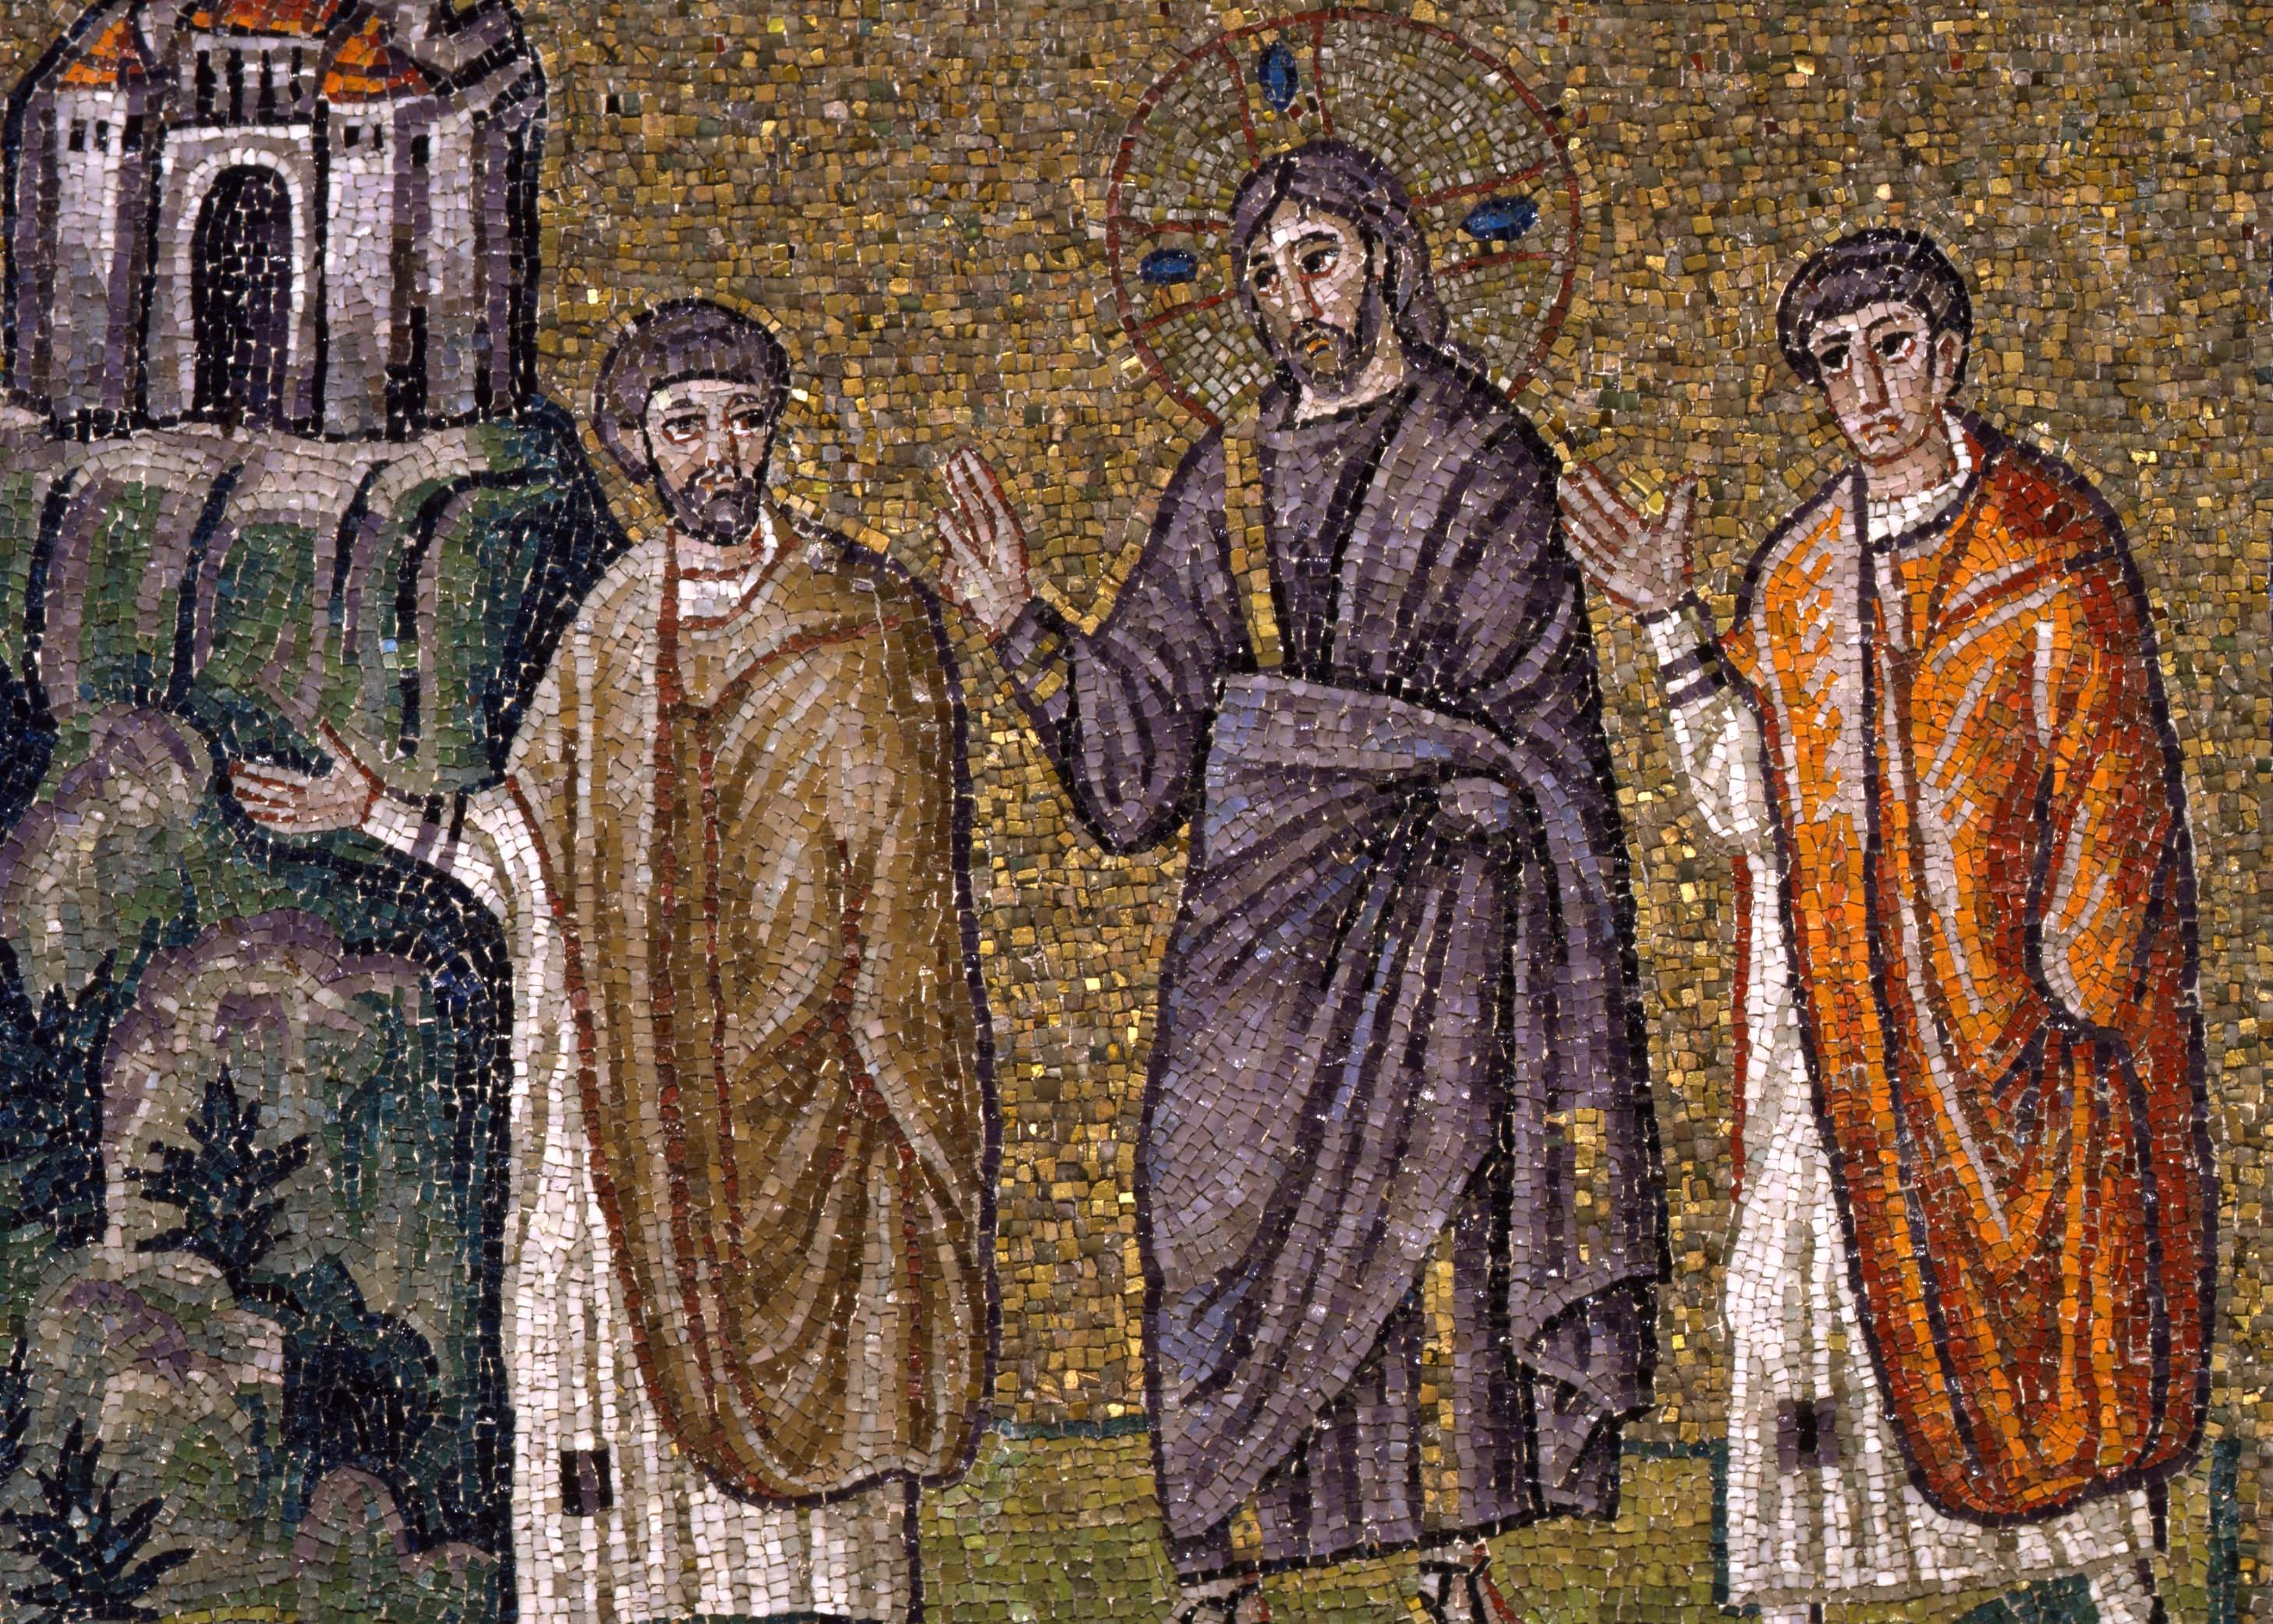
\includegraphics[width=8cm]{emmaus.jpg}
%\end{center}

\vfill

\begin{center}
%Ad usum et secundum consuetudines chori \guillemotright{}Conventus Choralis\guillemotleft.

%Editio Sancti Wolfgangi \annusEditionis
\end{center}

\pagebreak

\renewcommand{\headrulewidth}{0pt} % no horiz. rule at the header
\fancyhf{}
\pagestyle{fancy}

\pars{Oratio ante divinum Officium.}

\lettrine{{\color{red}A}}{peri,} Dómine, os meum ad benedicéndum nomen sanctum tuum:
munda quoque cor meum ab ómnibus vanis, pervérsis, et aliénis
cogitatiónibus:
intelléctum illúmina, afféctum inflámma,
ut digne, atténte ac devóte hoc Offícium recitáre váleam,
et exaudíri mérear ante conspéctum Divínæ Maiestátis tuæ.
Per Christum, Dóminum nostrum.
\Rbardot{} Amen.

Dómine, in unióne illíus divínæ intentiónis,
qua ipse in terris laudes Deo persolvísti,
has tibi Horas \rubricatum{(vel \textnormal{hanc tibi Horam})} persólvo.

%\trOratioAnteOfficium

\vfill

\pars{Oratio post divinum Officium.}

\rubrica{
  Orationem sequentem devote post Officium recitantibus
  Leo Papa X. defectus, et culpas in eo persolvendo ex humana
  fragilitate contractas, indulsit, et dicitur flexis genibus.
}

\lettrine{{\color{red}S}}{acrosánctæ} et indivíduæ Trinitáti,
crucifíxi Dómini nostri Iesu Christi humanitáti,
beatíssimæ et gloriosíssimæ sempérque Vírginis Maríæ
fecúndæ integritáti, 
et ómnium Sanctórum universitáti
sit sempitérna laus, honor, virtus et glória
ab omni creatúra,
nobísque remíssio ómnium peccatórum,
per infiníta sǽcula sæculórum.
\Rbardot{} Amen.

\noindent \Vbardot{} Beáta víscera Maríæ Virginis, quæ portavérunt
ætérni Patris Fílium.\\
\Rbardot{} Et beáta úbera, quæ lactavérunt Christum Dominum.

\rubrica{Et dicitur secreto \textnormal{Pater noster.} et \textnormal{Ave María.}}

%\trOratioPostOfficium

\vfill

\hora{Ad I. Vesperas.} %%%%%%%%%%%%%%%%%%%%%%%%%%%%%%%%%%%%%%%%%%%%%%%%%%%%%
%\sideThumbs{I. Vesperæ}

\cantusSineNeumas

\vspace{0.5cm}
\grechangedim{interwordspacetext}{0.18 cm plus 0.15 cm minus 0.05 cm}{scalable}%
\cuminitiali{}{temporalia/deusinadiutorium-solemnis.gtex}
\grechangedim{interwordspacetext}{0.22 cm plus 0.15 cm minus 0.05 cm}{scalable}%

\vfill
\pagebreak

\pars{Psalmus 1.}

\vspace{-0.4cm}

\antiphona{VII c\textsuperscript{2}}{temporalia/ant-alleluia1.gtex}

\scriptura{Psalmus 144, 10-21.}

\initiumpsalmi{temporalia/ps144ii-initium-vii-c2-auto.gtex}

%\psalmusEtTranslatioT{temporalia/ps144ii-comb.tex}{10cm}
\input{temporalia/ps144ii.tex}

\vspace{-1cm}

\vfill
\pagebreak

\pars{Psalmus 2.}

\scriptura{Psalmus 145.}

\initiumpsalmi{temporalia/ps145-initium-vii-c2-auto.gtex}

%\psalmusEtTranslatioT{temporalia/ps145-comb.tex}{10cm}
\input{temporalia/ps145.tex}

\vfill
\pagebreak

\pars{Psalmus 3.}

\scriptura{Psalmus 146.}

\initiumpsalmi{temporalia/ps146-initium-vii-c2-auto.gtex}

%\psalmusEtTranslatioT{temporalia/ps146-comb.tex}{10cm}
\input{temporalia/ps146.tex}

\vfill
\pagebreak

\pars{Psalmus 4.}

\scriptura{Psalmus 147.}

\initiumpsalmi{temporalia/ps147-initium-vii-c2-auto.gtex}

%\psalmusEtTranslatioT{temporalia/ps147-comb.tex}{10cm}
\input{temporalia/ps147.tex}

\vfill

\vspace{-6mm}

\antiphona{}{temporalia/ant-alleluia1.gtex} % repeat the antiphon - new page

\vfill
\pagebreak

\pars{Capitulum.} \scriptura{1 Petr. 2, 21-22}

\grechangedim{interwordspacetext}{0.12 cm plus 0.15 cm minus 0.05 cm}{scalable}%
\cuminitiali{}{temporalia/capitulum-CarissimiChristusPassus.gtex}
\grechangedim{interwordspacetext}{0.22 cm plus 0.15 cm minus 0.05 cm}{scalable}%

% preklad Jeruz. bible
%\trCapituliI

\vfill

\pars{Responsorium breve.} \scriptura{Lc. 24, 34}

\cuminitiali{VI}{temporalia/respbr-vesp.gtex}

%\trResp

\vfill
\pagebreak

\pars{Hymnus}

\cuminitiali{VIII}{temporalia/hym-AdCoenam.gtex}
\vspace{-3mm}
%\begin{translatioMulticol}{4}
U~Beránkovy hostiny\\
oděni rouchy bílými,\\
když Rudým mořem prošli jsme,\\
Vladaři Kristu zpívejme.\\
\\
Když jeho tělem posvátným,\\
na kříži obětovaným,\\
se sytíme a~pijeme\\
jeho krev, v~Bohu žijeme.\columnbreak

Chráněni tímto pokrmem\\
před smrtonosným andělem,\\
svrhli jsme z~beder kruté jho\\
tyrana bezohledného.\\
\\
Kristus je naší paschou teď,\\
on sám se vydal za oběť\\
a~místo přesnic našim rtům\\
své tělo dává za pokrm.\columnbreak

Tys, nejčistější Oběti,\\
zlomila vládu podsvětí.\\
Z~otroctví lid je vykoupen,\\
odměna žití kyne všem.\\
\\
Hle, Kristus, když vstal ze hrobu,\\
jde z~pekel v~slavném průvodu\\
a~brány nebes otevřev,\\
vládce tmy vleče v~okovech.\columnbreak

Buď věčně, Kriste, věrným svým\\
plesáním velikonočním.\\
Nás, milostí tvou vzkříšené,\\
vem k~oslavě své vítězné. \\
\\
Sláva tobě, Pane,\\
jenž jsi vstal z~mrtvých,\\
s~Otcem i~Svatým Duchem\\
na věčné věky.\\
Amen.
\end{translatioMulticol}


\vfill
\pagebreak

\pars{Versus.} \scriptura{Lc. 24, 29}

% Versus. %%%
\sineinitiali{temporalia/versus-mane.gtex}

%\noindent \trVersus

\vfill
\pagebreak

\pars{Canticum B. Mariæ V.} \scriptura{Cf. Io. 10, 2.14; Io. 14, 6; \textbf{H242}}

\vspace{-6mm}

{
\grechangedim{interwordspacetext}{0.18 cm plus 0.15 cm minus 0.05 cm}{scalable}%
\antiphona{VIII G\textsuperscript{2}}{temporalia/ant-egosumpastorovium.gtex}
\grechangedim{interwordspacetext}{0.22 cm plus 0.15 cm minus 0.05 cm}{scalable}%
}

%\trAntIMagnificat

\vspace{-4mm}

\scriptura{Lc. 1, 46-55}

\cantusSineNeumas
\initiumpsalmi{temporalia/magnificat-initium-viii-G2.gtex}

%\vspace{-7mm}

%\psalmusEtTranslatioT{temporalia/magnificat-III-comb.tex}{10.2cm}
\input{temporalia/magnificat-III.tex}

\vspace{-1cm}

\vfill
\pagebreak

%\sideThumbs{{\scriptsize{}Fine horarum}}

\anteOrationem

\pagebreak

% Oratio. %%%
\cuminitiali{}{temporalia/oratio2.gtex}

\vspace{-1mm}
%\trOrationisI

\vfill

\rubrica{Hebdomadarius dicit iterum Dominus vobiscum. Postea cantatur a cantore:}
\vspace{2mm}

\cuminitiali{VII}{temporalia/benedicamus-tempore-paschali.gtex}

\vspace{1mm}

\vfill
\pagebreak

\hora{Ad Matutinum.} %%%%%%%%%%%%%%%%%%%%%%%%%%%%%%%%%%%%%%%%%%%%%%%%%%%%%
%\sideThumbs{Matutinum}

\vspace{2mm}

\cuminitiali{}{temporalia/dominelabiamea.gtex}

\vspace{2mm}

\pars{Invitatorium.} \scriptura{Lc. 24, 34; Psalmus 94; \textbf{H232}}

\vspace{-6mm}

\antiphona{VI}{temporalia/inv-surrexitdominusvere.gtex}

\vfill
\pagebreak

\pars{Hymnus.}

\vspace{-5mm}

\scriptura{\textbf{AR454}}

{
\grechangedim{interwordspacetext}{0.30 cm plus 0.15 cm minus 0.05 cm}{scalable}%
\antiphona{IV}{temporalia/hym-RexSempiterne.gtex}
\grechangedim{interwordspacetext}{0.32 cm plus 0.15 cm minus 0.05 cm}{scalable}%
}
%{
%\vspace{-5mm}
%\setlength{\columnsep}{0pt} % prostor mezi sloupci
%\input{hym-RexSempiterne-bohtext.tex}
%\setlength{\columnsep}{30pt} % prostor mezi sloupci
%}

\vfill
\pagebreak

\subhora{In I. Nocturno}

\pars{Psalmus 1.} \scriptura{\textbf{H230}}

%\vspace{-5mm}

\antiphona{V a}{temporalia/ant-alleluialapis.gtex}

%\vspace{-5mm}

\scriptura{Ps. 1}

%\vspace{-2mm}

\initiumpsalmi{temporalia/ps1-initium-v-a-auto.gtex}

%\psalmusEtTranslatioT{temporalia/ps1-comb.tex}{10cm}

\input{temporalia/ps1.tex}

\vfill
\pagebreak

\pars{Psalmus 2.}

\scriptura{Ps. 2}

\initiumpsalmi{temporalia/ps2-initium-v-a-auto.gtex}

%\psalmusEtTranslatioT{temporalia/ps2-comb.tex}{10cm}

\input{temporalia/ps2.tex}

\vfill
\pagebreak

\pars{Psalmus 3.}

\scriptura{Ps. 3}

\initiumpsalmi{temporalia/ps3-initium-v-a-auto.gtex}

%\psalmusEtTranslatioT{temporalia/ps3-comb.tex}{10cm}

\input{temporalia/ps3.tex}

\vfill

\antiphona{}{temporalia/ant-alleluialapis.gtex}

\vfill
\pagebreak

\noindent \Vbardot{} Surréxit Dóminus de sepúlcro, allelúia.
\noindent \Rbardot{} Qui pro nobis pepéndit in ligno, allelúia.

\noindent Pater noster.

\pars{Absolutio.}

\cuminitiali{}{temporalia/absolutio-exaudi.gtex}

\cuminitiali{}{temporalia/benedictio-solemn-benedictione.gtex}

\vfill
\pagebreak

\pars{Lectio I.} \scriptura{Ac. 13, 13-20}

\noindent De Actibus Apostolórum.

\noindent Cum a Papho navigássent Paulus et qui cum eo erant, venérunt Pergen Pamphýliæ. Ioánnes autem discédens ab eis, revérsus est Ierosólymam. Illi vero pertranseúntes Pergen, venérunt Antiochíam Pisídiæ: et ingréssi synagógam die sabbatórum, sedérunt. Post lectiónem autem legis et prophetárum, misérunt príncipes synagógæ ad eos, dicéntes: Viri fratres, si quis est in vobis sermo exhortatiónis ad plebem, dícite. Surgens autem Paulus, et manu siléntium indícens, ait: Viri Israëlítæ, et qui timétis Deum, audíte: Deus plebis Israël elégit patres nostros, et plebem exaltávit cum essent íncolæ in terra Ægýpti, et in brácchio excélso edúxit eos ex ea, et per quadragínta annórum tempus mores eórum sustínuit in desérto. Et déstruens gentes septem in terra Chánaan, sorte distríbuit eis terram eórum, quasi post quadringéntos et quinquagínta annos: et post hæc dedit iúdices, usque ad Sámuel prophétam.

\noindent \Vbardot{} Tu autem, Dómine, miserére nobis.
\noindent \Rbardot{} Deo grátias.

\vfill
\pagebreak

\pars{Responsorium 1.} \scriptura{\Rbardot{} Mt. 28, 2; \Vbardot{} Bed. Ven. «In Marc. 4.16»; \textbf{H228}}

\vspace{-5mm}

\responsorium{III}{temporalia/resp-angelusdominidescendit.gtex}{}

\vfill
\pagebreak

\cuminitiali{}{temporalia/benedictio-solemn-unigenitus.gtex}

\vspace{7mm}

\pars{Lectio II.} \scriptura{Ac. 13, 21-25}

\noindent Et exínde postulavérunt regem: et dedit illis Deus Saul fílium Cis, virum de tribu Béniamin, annis quadragínta: et amóto illo, suscitávit illis David regem: cui testimónium pérhibens, dixit: Invéni David fílium Iesse, virum secúndum cor meum, qui fáciet omnes voluntátes meas. Huius Deus ex sémine secúndum promissiónem edúxit Israël salvatórem Iesum, prædicánte Ioánne ante fáciem advéntus eius baptísmum pœniténtiæ omni pópulo Israël. Cum impléret autem Ioánnes cursum suum, dicébat: Quem me arbitrámini esse, non sum ego: sed ecce venit post me, cuius non sum dignus calceaménta pedum sólvere.

\noindent \Vbardot{} Tu autem, Dómine, miserére nobis.
\noindent \Rbardot{} Deo grátias.

\vfill
\pagebreak

\pars{Responsorium 2.} \scriptura{\Rbardot{} Mt. 28, 5.6; \Vbardot{} Mc. 16, 6; \textbf{H229}}

\vspace{-5mm}

\responsorium{V}{temporalia/resp-angelusdominilocutus.gtex}{}

\vfill
\pagebreak

\cuminitiali{}{temporalia/benedictio-solemn-spiritus.gtex}

\vspace{7mm}

\pars{Lectio III.} \scriptura{Ac. 13, 26-33}

\noindent Viri fratres, fílii géneris Abraham, et qui in vobis timent Deum, vobis verbum salútis huius missum est. Qui enim habitábant Ierúsalem, et príncipes eius hunc ignorántes, et voces prophetárum quæ per omne sábbatum legúntur, iudicántes implevérunt, et nullam causam mortis inveniéntes in eo, petiérunt a Piláto ut interfícerent eum. Cumque consummássent ómnia quæ de eo scripta erant, deponéntes eum de ligno, posuérunt eum in monuménto. Deus vero suscitávit eum a mórtuis tértia die: qui visus est per dies multos his qui simul ascénderant cum eo de Galilǽa in Ierúsalem: qui usque nunc sunt testes eius ad plebem. Et nos vobis annuntiámus eam, quæ ad patres nostros repromíssio facta est: quóniam hanc Deus adimplévit fíliis nostris resúscitans Iesum, sicut et in psalmo secúndo scriptum est: Fílius meus es tu, ego hódie génui te.

\noindent \Vbardot{} Tu autem, Dómine, miserére nobis.
\noindent \Rbardot{} Deo grátias.

\vfill
\pagebreak

\pars{Responsorium 3.} \scriptura{\Rbardot{} Mc. 16, 1; \Vbardot{} ibid. 16, 2; \textbf{H229}}

\vspace{-5mm}

\responsorium{IV}{temporalia/resp-dumtransisset.gtex}{}

\vfill
\pagebreak

\subhora{In II. Nocturno}

\pars{Psalmus 4.} \scriptura{Io. 20, 15; \textbf{H241}}

%\vspace{-5mm}

\antiphona{V a}{temporalia/ant-alleluiaquem.gtex}

%\vspace{-5mm}

\scriptura{Ps. 8}

%A\vspace{-2mm}

\initiumpsalmi{temporalia/ps8-initium-v-a-auto.gtex}

%\psalmusEtTranslatioT{temporalia/ps8-comb.tex}{10cm}

\input{temporalia/ps8.tex}

\vfill
\pagebreak

\pars{Psalmus 5.}

\scriptura{Ps. 9, 2-11}

\initiumpsalmi{temporalia/ps9ii_xi-initium-v-a-auto.gtex}

%\psalmusEtTranslatioT{temporalia/ps9ii_xi-comb.tex}{10cm}

\input{temporalia/ps9ii_xi.tex}

\vfill
\pagebreak

\pars{Psalmus 6.}

\scriptura{Ps. 9, 12-21}

\initiumpsalmi{temporalia/ps9xii_xxi-initium-v-a-auto.gtex}

%\psalmusEtTranslatioT{temporalia/ps9xii_xxi-comb.tex}{10cm}

\input{temporalia/ps9xii_xxi.tex}

\vfill

\antiphona{}{temporalia/ant-alleluiaquem.gtex}

\vfill
\pagebreak

\noindent \Vbardot{} Surréxit Dóminus vere, allelúia.
\noindent \Rbardot{} Et appáruit Simóni, allelúia.

\noindent Pater noster.

\pars{Absolutio.}

\cuminitiali{}{temporalia/absolutio-ipsius.gtex}

\cuminitiali{}{temporalia/benedictio-solemn-deus.gtex}

\vfill
\pagebreak

\pars{Lectio IV.} \scriptura{Sermo 1 de Ascensione Domini, post initium}

\noindent Sermo sancti Leónis Papæ.

\noindent Hi dies, dilectíssimi, qui inter resurrectiónem Dómini ascensionémque fluxérunt, non otióso transiére decúrsu, sed magna in eis confirmáta sacraménta, magna sunt reveláta mystéria. In iis metus diræ mortis aufértur, et non solum ánimæ, sed étiam carnis immortálitas declarátur. In iis per insufflatiónem Dómini infúnditur Apóstolis ómnibus Spíritus Sanctus: et beáto Apóstolo Petro supra céteros, post regni claves, ovílis Domínici cura mandátur.

\noindent \Vbardot{} Tu autem, Dómine, miserére nobis.
\noindent \Rbardot{} Deo grátias.

\vfill
\pagebreak

\pars{Responsorium 4.} \scriptura{\Rbardot{} Mt. 28, 1 \& Cantor; \Vbardot{} ibidem; \textbf{H232}}

\vspace{-5mm}

\responsorium{VIII}{temporalia/resp-mariamagdalene.gtex}{}

\vfill
\pagebreak

\cuminitiali{}{temporalia/benedictio-solemn-christus.gtex}

\vspace{7mm}

\pars{Lectio V.}

\noindent In iis diébus, duóbus discípulis tértius in via Dóminus comes iúngitur, et ad omnem nostræ ambiguitátis calíginem detergéndam, pavéntium ac trepidántium tárditas increpátur. Flammam fídei illumináta corda concípiunt: et quæ erant tépida, reseránte Scriptúras Dómino, efficiúntur ardéntia. In fractióne quoque panis, convescéntium aperiúntur obtútus: multo felícius eórum óculis patefáctis, quibus natúræ suæ manifestáta est glorificátio, quam illórum géneris nostri príncipum, quibus prævaricatiónis suæ est ingésta confúsio.

\noindent \Vbardot{} Tu autem, Dómine, miserére nobis.
\noindent \Rbardot{} Deo grátias.

\vfill
\pagebreak

\pars{Responsorium 5.} \scriptura{\Rbardot{} Io. 10, 11; \Vbardot{} I Cor. 5, 7; \textbf{H237}}

\vspace{-5mm}

\responsorium{I}{temporalia/resp-surrexitpastor.gtex}{}

\vfill
\pagebreak

\cuminitiali{}{temporalia/benedictio-solemn-ignem.gtex}

\vspace{7mm}

\pars{Lectio VI.}

\noindent Inter hæc autem, aliáque mirácula, cum discípuli trépidis cogitatiónibus æstuárent, et apparuísset in médio eórum Dóminus, dixissétque, Pax vobis: ne hoc remanéret in eórum opiniónibus, quod volvebátur in córdibus (putábant enim se spíritum vidére, non carnem) redárguit cogitatiónes a veritáte discórdes: íngerit dubitántium óculis manéntia in mánibus suis et pédibus crucis signa; et ut diligéntius pertractétur, invítat. Quia ad sanánda infidélium cordium vúlnera, clavórum et lánceæ erant serváta vestígia: ut non dúbia fide, sed constantíssima sciéntia tenerétur, eam natúram in Dei Patris consessúram throno, quæ iacúerat in sepúlcro.

\noindent \Vbardot{} Tu autem, Dómine, miserére nobis.
\noindent \Rbardot{} Deo grátias.

\vfill
\pagebreak

\pars{Responsorium 6.} \scriptura{\Rbardot{} Ac. 4, 33; \Vbardot{} ibid. 4, 31; \textbf{H234}}

\vspace{-5mm}

\responsorium{III}{temporalia/resp-virtutemagna.gtex}{}

\vfill
\pagebreak

\subhora{In III. Nocturno}

\pars{Psalmus 7.} \scriptura{Cf. Io. 20, 15; \textbf{H241}}

\vspace{-5mm}

\antiphona{V a}{temporalia/ant-alleluianoli.gtex}

\vspace{-4mm}

\scriptura{Ps. 9, 22-32}

%\vspace{-2mm}

\initiumpsalmi{temporalia/ps9xxii_xxxii-initium-v-a-auto.gtex}

%\psalmusEtTranslatioT{temporalia/ps9xxii_xxxii-comb.tex}{10cm}

\input{temporalia/ps9xxii_xxxii.tex}

\vfill
\pagebreak

\pars{Psalmus 8.}

\scriptura{Ps. 9, 33-39}

\initiumpsalmi{temporalia/ps9xxxiii_xxxix-initium-v-a-auto.gtex}

%\psalmusEtTranslatioT{temporalia/ps9xxxiii_xxxix-comb.tex}{10cm}

\input{temporalia/ps9xxxiii_xxxix.tex}

\vfill
\pagebreak

\pars{Psalmus 9.}

\scriptura{Ps. 10}

\initiumpsalmi{temporalia/ps10-initium-v-a-auto.gtex}

%\psalmusEtTranslatioT{temporalia/ps10-comb.tex}{10cm}

\input{temporalia/ps10.tex}

\vfill

\antiphona{}{temporalia/ant-alleluianoli.gtex}

\vfill
\pagebreak

\noindent \Vbardot{} Gavísi sunt discípuli, allelúia.
\noindent \Rbardot{} Viso Dómino, allelúia.

\noindent Pater noster.

\pars{Absolutio.}

\cuminitiali{}{temporalia/absolutio-avinculis.gtex}

\cuminitiali{}{temporalia/benedictio-solemn-evangelica.gtex}

\vfill
\pagebreak

\pars{Lectio VII.} \scriptura{Io. 10, 11-16}

\noindent Léctio sancti Evangélii secúndum Ioánnem.

\noindent In illo témpore: Dixit Iesus pharisǽis: Ego sum pastor bonus. Bonus pastor ánimam suam dat pro óvibus suis. Et réliqua.

\scriptura{Homilia 14 in Evangelia}

\noindent Homilía sancti Gregórii Papæ.

\noindent Audístis, fratres caríssimi, ex lectióne evangélica eruditiónem vestram: audístis et perículum nostrum. Ecce enim is, qui non ex accidénti dono, sed essentiáliter bonus est, dicit: Ego sum pastor bonus. Atque eiúsdem bonitátis formam, quam nos imitémur, adiúngit, dicens: Bonus pastor ánimam suam ponit pro óvibus suis. Fecit quod mónuit: osténdit quod iussit. Bonus pastor pro óvibus suis ánimam suam pósuit, ut in sacraménto nostro corpus suum et sánguinem vérteret, et oves quas redémerat, carnis suæ aliménto satiáret.

\noindent \Vbardot{} Tu autem, Dómine, miserére nobis.
\noindent \Rbardot{} Deo grátias.

\vfill
\pagebreak

\pars{Responsorium 7.} \scriptura{\Rbardot{} Cant. 4, 11; \Vbardot{} Parab. 14, 33; \textbf{H236}}

\vspace{-5mm}

\responsorium{VII}{temporalia/resp-deoreprudentis.gtex}{}

\vfill
\pagebreak

\cuminitiali{}{temporalia/benedictio-solemn-divinum.gtex}

\vspace{7mm}

\pars{Lectio VIII.}

\noindent Osténsa nobis est de contémptu mortis via, quam sequámur: appósita est forma, cui imprimámur. Primum nobis est, exterióra nostra misericórditer óvibus eius impéndere: postrémum vero, si necésse sit, étiam mortem nostram pro eísdem óvibus ministráre. A primo autem hoc mínimo pervenítur ad postrémum maius. Sed cum incomparabíliter longe sit mélior ánima, qua vívimus, quam terréna substántia, quam extérius possidémus: qui non dat pro óvibus substántiam suam, quando pro his datúrus est ánimam suam?

\noindent \Vbardot{} Tu autem, Dómine, miserére nobis.
\noindent \Rbardot{} Deo grátias.

\vfill
\pagebreak

\pars{Responsorium 8.} \scriptura{\Rbardot{} Io. 20, 19-20; \Vbardot{} ibid. 20, 19; \textbf{H232}}

\vspace{-5mm}

\responsorium{VII}{temporalia/resp-surgensjesus.gtex}{}

\vfill
\pagebreak

\cuminitiali{}{temporalia/benedictio-solemn-adsocietatem.gtex}

\vspace{7mm}

\pars{Lectio IX.}

\noindent Et sunt nonnúlli, qui dum plus terrénam substántiam quam oves díligunt, mérito nomen pastóris perdunt: de quibus prótinus súbditur: Mercenárius autem, et qui non est pastor, cuius non sunt oves própriæ, videt lupum veniéntem, et dimíttet oves, et fugit. Non pastor, sed mercenárius vocátur, qui non pro amóre íntimo oves Domínicas, sed ad temporáles mercédes pascit. Mercenárius quippe est, qui locum quidem pastóris tenet, sed lucra animárum non quærit: terrénis cómmodis ínhiat, honóre prælatiónis gaudet, temporálibus lucris páscitur, impénsa sibi ab homínibus reveréntia lætátur.

\noindent \Vbardot{} Tu autem, Dómine, miserére nobis.
\noindent \Rbardot{} Deo grátias.

\vfill
\pagebreak

% Te Deum

%\pars{Hymnus Ambrosianus}

\vspace{-5mm}

{
\grechangedim{interwordspacetext}{0.22 cm plus 0.15 cm minus 0.05 cm}{scalable}%
\cuminitiali{III}{temporalia/tedeum-solemnis.gtex}
\grechangedim{interwordspacetext}{0.32 cm plus 0.15 cm minus 0.05 cm}{scalable}%
}

\vfill
\pagebreak

\rubrica{Reliqua omittuntur, nisi Laudes separandæ sint.}

\pars{Oratio}

\noindent \Vbardot{} Dómine, exáudi oratiónem meam.

\noindent \Rbardot{} Et clamor meus ad te véniat.

Orémus:

\noindent Deus, qui in Fílii tui humilitáte iacéntem mundum erexísti: \gredagger{} fidélibus tuis perpétuam concéde lætítiam; \grestar{} ut quos perpétuæ mortis eripuísti cásibus, gáudiis fácias pérfrui sempitérnis. Per eúmdem Dóminum.

\noindent \Rbardot{} Amen.

\vspace{7mm}

\pars{Conclusio}

\noindent \Vbardot{} Dómine, exáudi oratiónem meam.

\noindent \Rbardot{} Et clamor meus ad te véniat.

\noindent \Vbardot{} Benedicámus Dómino, allelúia, allelúia.

\noindent \Rbardot{} Deo grátias, allelúia, allelúia.

\noindent \Vbardot{} Fidélium ánimæ per misericórdiam Dei requiéscant in pace.

\noindent \Rbardot{} Amen.

\vfill
\pagebreak

\hora{Ad Laudes.} %%%%%%%%%%%%%%%%%%%%%%%%%%%%%%%%%%%%%%%%%%%%%%%%%%%%%
%\sideThumbs{Laudes}

\cantusSineNeumas

\vspace{0.5cm}
\grechangedim{interwordspacetext}{0.18 cm plus 0.15 cm minus 0.05 cm}{scalable}%
\cuminitiali{}{temporalia/deusinadiutorium-alter.gtex}
\grechangedim{interwordspacetext}{0.22 cm plus 0.15 cm minus 0.05 cm}{scalable}%

\vfill
%\pagebreak

\pars{Psalmus 1.}

\vspace{-0.4cm}

\antiphona{VIII G}{temporalia/ant-alleluia2.gtex}

\scriptura{Psalmus 92.}

\initiumpsalmi{temporalia/ps92-initium-viii-g-auto.gtex}

%\psalmusEtTranslatioT{temporalia/ps92-comb.tex}{10cm}
\input{temporalia/ps92.tex}

\vspace{-1cm}

\vfill
\pagebreak

\pars{Psalmus 2.}

\scriptura{Psalmus 99.}

\initiumpsalmi{temporalia/ps99-initium-viii-g-auto.gtex}

%\psalmusEtTranslatioT{temporalia/ps99-comb.tex}{10cm}
\input{temporalia/ps99.tex}

\vfill
\pagebreak

\pars{Psalmus 3.}

\scriptura{Psalmus 62.}

\initiumpsalmi{temporalia/ps62-initium-viii-g-auto.gtex}

%\psalmusEtTranslatioT{temporalia/ps62-comb.tex}{10cm}
\input{temporalia/ps62.tex}

\vfill

\vspace{-6mm}

\antiphona{}{temporalia/ant-alleluia2.gtex} % repeat the antiphon - new page

\vfill
\pagebreak

\pars{Psalmus 4.}

\vspace{-0.4cm}

\antiphona{VI F}{temporalia/ant-surrexitchristus.gtex}

\scriptura{Canticum trium puerorum, Dan. 3, 57-88 et 56}

\initiumpsalmi{temporalia/dan3-initium-vi-F-auto.gtex}

%\psalmusEtTranslatioT{temporalia/dan3-comb.tex}{10cm}
\input{temporalia/dan3.tex}

\vfill

\vspace{-6mm}

\antiphona{}{temporalia/ant-surrexitchristus.gtex} % repeat the antiphon - new page

\vfill
\pagebreak

\pars{Psalmus 5.}

\vspace{-0.4cm}

\antiphona{VI F}{temporalia/ant-alleluia3.gtex}

\scriptura{Psalmus 148.}

\initiumpsalmi{temporalia/ps148-initium-vi-F-auto.gtex}

%\psalmusEtTranslatioT{temporalia/ps148-comb.tex}{10cm}
\input{temporalia/ps148.tex}

\rubrica{Hic non dicitur Gloria Patri.}

\vfill
\pagebreak

%
\scriptura{Psalmus 149.}

\initiumpsalmi{temporalia/ps149-initium-vi-F-auto.gtex}

%\psalmusEtTranslatioT{temporalia/ps149-comb.tex}{10cm}
\input{temporalia/ps149.tex}

\rubrica{Hic non dicitur Gloria Patri.}

\vfill
\pagebreak

%
\scriptura{Psalmus 150.}

\initiumpsalmi{temporalia/ps150-initium-vi-F-auto.gtex}

%\psalmusEtTranslatioT{temporalia/ps150-comb.tex}{10cm}
\input{temporalia/ps150.tex}

\vfill

\vspace{-6mm}

\antiphona{}{temporalia/ant-alleluia3.gtex} % repeat the antiphon - new page

\vfill
\pagebreak

\pars{Capitulum.} \scriptura{1 Petr. 2, 21-22}

\grechangedim{interwordspacetext}{0.12 cm plus 0.15 cm minus 0.05 cm}{scalable}%
\cuminitiali{}{temporalia/capitulum-CarissimiChristusPassus.gtex}
\grechangedim{interwordspacetext}{0.22 cm plus 0.15 cm minus 0.05 cm}{scalable}%

% preklad Jeruz. bible
%\trCapituliI

\vfill

\pars{Responsorium breve.} \scriptura{Cf. Mt. 28, 6; Cf. Gal. 3, 13}

\cuminitiali{VI}{temporalia/respbr-laud.gtex}

%\trResp

\vfill
\pagebreak

\pars{Hymnus}

\cuminitiali{VIII}{temporalia/hym-AuroraLucis.gtex}
\vspace{-3mm}
%\input{hym-AuroraLucis-bohtext.tex}

\vfill
%\pagebreak

\pars{Versus.}

% Versus. %%%
\sineinitiali{temporalia/versus-inresurrectione.gtex}

%\noindent \trVersus

\vfill
\pagebreak

\pars{Canticum Zachariæ.} \scriptura{Cf. Io. 10, 2.14; Io. 14, 6; \textbf{H242}}

\vspace{-7mm}

{
\grechangedim{interwordspacetext}{0.18 cm plus 0.15 cm minus 0.05 cm}{scalable}%
\antiphona{I D}{temporalia/ant-egosumpastorovium.gtex}
\grechangedim{interwordspacetext}{0.22 cm plus 0.15 cm minus 0.05 cm}{scalable}%
}

%\trAntIMagnificat

\vspace{-3mm}

\scriptura{Lc. 1, 68-79}

\vspace{-3mm}

\cantusSineNeumas
\initiumpsalmi{temporalia/benedictus-initium-viiisoll-G2-auto.gtex}

%\psalmusEtTranslatioT{temporalia/benedictus-II-comb.tex}{10.2cm}
\input{temporalia/benedictus-II.tex}

\vspace{-1cm}

\vfill
\pagebreak

%\sideThumbs{{\scriptsize{}Fine horarum}}

\anteOrationem

\pagebreak

% Oratio. %%%
\cuminitiali{}{temporalia/oratio2.gtex}

\vspace{-1mm}
%\trOrationisI

\vfill

\rubrica{Hebdomadarius dicit iterum Dominus vobiscum. Postea cantatur a cantore:}
\vspace{2mm}

\cuminitiali{VII}{temporalia/benedicamus-tempore-paschali.gtex}

\vspace{1mm}

\vfill
\pagebreak

\hora{Ad II. Vesperas.} %%%%%%%%%%%%%%%%%%%%%%%%%%%%%%%%%%%%%%%%%%%%%%%%%%%%%
%\sideThumbs{II. Vesperæ}

\cantusSineNeumas

\vspace{0.5cm}
\grechangedim{interwordspacetext}{0.18 cm plus 0.15 cm minus 0.05 cm}{scalable}%
\cuminitiali{}{temporalia/deusinadiutorium-solemnis.gtex}
\grechangedim{interwordspacetext}{0.22 cm plus 0.15 cm minus 0.05 cm}{scalable}%

\vfill
%\pagebreak

\vspace{-2mm}

\pars{Psalmus 1.}

\vspace{-0.4cm}

\antiphona{VII c\textsuperscript{2}}{temporalia/ant-alleluia4.gtex}

\vspace{-4mm}

\scriptura{Psalmus 109.}

\initiumpsalmi{temporalia/ps109-initium-vii-c2-auto.gtex}

%\psalmusEtTranslatioT{temporalia/ps109-comb.tex}{10cm}
\input{temporalia/ps109.tex}

\vspace{-1cm}

\vfill
\pagebreak

\pars{Psalmus 2.}

\scriptura{Psalmus 110.}

\initiumpsalmi{temporalia/ps110-initium-vii-c2-auto.gtex}

%\psalmusEtTranslatioT{temporalia/ps110-comb.tex}{10cm}
\input{temporalia/ps110.tex}

\vfill
\pagebreak

\pars{Psalmus 3.}

\scriptura{Psalmus 111.}

\initiumpsalmi{temporalia/ps111-initium-vii-c2-auto.gtex}

%\psalmusEtTranslatioT{temporalia/ps111-comb.tex}{10cm}
\input{temporalia/ps111.tex}

\vfill
\pagebreak

\pars{Psalmus 4.}

\scriptura{Psalmus 112.}

\initiumpsalmi{temporalia/ps112-initium-vii-c2-auto.gtex}

%\psalmusEtTranslatioT{temporalia/ps112-comb.tex}{10cm}
\input{temporalia/ps112.tex}

\vfill

\vspace{-6mm}

\antiphona{}{temporalia/ant-alleluia4.gtex} % repeat the antiphon - new page

\vfill
\pagebreak

\pars{Capitulum.} \scriptura{1 Petr. 2, 21-22}

\grechangedim{interwordspacetext}{0.12 cm plus 0.15 cm minus 0.05 cm}{scalable}%
\cuminitiali{}{temporalia/capitulum-CarissimiChristusPassus.gtex}
\grechangedim{interwordspacetext}{0.22 cm plus 0.15 cm minus 0.05 cm}{scalable}%

% preklad Jeruz. bible
%\trCapituliI

\vfill

\pars{Responsorium breve.} \scriptura{Lc. 24, 34}

\cuminitiali{VI}{temporalia/respbr-vesp.gtex}

%\trResp

\vfill
\pagebreak

\pars{Hymnus}

\cuminitiali{VIII}{temporalia/hym-AdCoenam.gtex}
\vspace{-3mm}
%\begin{translatioMulticol}{4}
U~Beránkovy hostiny\\
oděni rouchy bílými,\\
když Rudým mořem prošli jsme,\\
Vladaři Kristu zpívejme.\\
\\
Když jeho tělem posvátným,\\
na kříži obětovaným,\\
se sytíme a~pijeme\\
jeho krev, v~Bohu žijeme.\columnbreak

Chráněni tímto pokrmem\\
před smrtonosným andělem,\\
svrhli jsme z~beder kruté jho\\
tyrana bezohledného.\\
\\
Kristus je naší paschou teď,\\
on sám se vydal za oběť\\
a~místo přesnic našim rtům\\
své tělo dává za pokrm.\columnbreak

Tys, nejčistější Oběti,\\
zlomila vládu podsvětí.\\
Z~otroctví lid je vykoupen,\\
odměna žití kyne všem.\\
\\
Hle, Kristus, když vstal ze hrobu,\\
jde z~pekel v~slavném průvodu\\
a~brány nebes otevřev,\\
vládce tmy vleče v~okovech.\columnbreak

Buď věčně, Kriste, věrným svým\\
plesáním velikonočním.\\
Nás, milostí tvou vzkříšené,\\
vem k~oslavě své vítězné. \\
\\
Sláva tobě, Pane,\\
jenž jsi vstal z~mrtvých,\\
s~Otcem i~Svatým Duchem\\
na věčné věky.\\
Amen.
\end{translatioMulticol}


\vfill
\pagebreak

\pars{Versus.} \scriptura{Lc. 24, 29}

% Versus. %%%
\sineinitiali{temporalia/versus-mane.gtex}

%\noindent \trVersus

\vfill
\pagebreak

\pars{Canticum B. Mariæ V.} \scriptura{Cf. Io. 10, 14}

\vspace{-4mm}

{
\grechangedim{interwordspacetext}{0.18 cm plus 0.15 cm minus 0.05 cm}{scalable}%
\antiphona{III a}{temporalia/ant-egosumpastorbonus.gtex}
\grechangedim{interwordspacetext}{0.22 cm plus 0.15 cm minus 0.05 cm}{scalable}%
}

%\trAntIMagnificat

\vspace{-3mm}

\scriptura{Lc. 1, 46-55}

\cantusSineNeumas
\initiumpsalmi{temporalia/magnificat-initium-iii-a.gtex}

%\vspace{-7mm}

%\psalmusEtTranslatioT{temporalia/magnificat-IV-comb.tex}{10.2cm}
\input{temporalia/magnificat-IV.tex}

\vspace{-1cm}

\vfill
\pagebreak

%\sideThumbs{{\scriptsize{}Fine horarum}}

\anteOrationem

\pagebreak

% Oratio. %%%
\cuminitiali{}{temporalia/oratio2.gtex}

\vspace{-1mm}
%\trOrationisI

\vfill

\rubrica{Hebdomadarius dicit iterum Dominus vobiscum. Postea cantatur a cantore:}
\vspace{2mm}

\cuminitiali{VII}{temporalia/benedicamus-tempore-paschali.gtex}

\vspace{1mm}

\newpage
\RemoveSideThumbs
\pagestyle{empty}

\pars{Antiphona finalis B. M. V. pro Tempore Paschali.}

\cuminitiali{VI}{temporalia/an_regina_caeli_simplex.gtex}
%\trReginaCaeli

%%% COLOPHON
%\vfill

%Fontes.
%Textus et cantus officii divini secundum
%Antiphonale Sacrosanctæ Romanæ Eclesiæ Pro Diurnis Horis, Romæ 1912, præter:
%hymni et responsoria breve secundum Antiphonale Monasticum pro Diurnis Horis,
%Solesmis 1934. /
%Translatio capituli sumpta est ex: Jeruzalémská bible, Praha-Kostelní Vydří 2009. /
%Translationes psalmorum ex Hejčl Jan: Žaltář čili Kniha žalmů, Praha 1922. /
%Neumæ super canto officii divini de codice Hartker, Stiftsbibl. 391.

%Collaborantes.
%Textus latinos cantusque transcripsit et omnem laborem typographicum peregit
%Jakub Jelínek. /
%Psalmos in lingua bohemica de libro transcripserunt Barbora Maturová et idem Jakub Jelínek. /
%Václav Ondráček textus responsoriorum in linguam bohemicam transtulit. /
%Mons. Jiří Reinsberg \olddag{} et Jana Kuběnová textus deprecationum in linguam bohemicam transtulerunt. /
%Zbyněk Šír et Filip Srovnal librum istum præparare mandaverunt et laborem exprobrationibus
%utilissimis comitabantur.

%Instrumenta adhibita.
%LuaTeX, %http://www.luatex.org /
%Gregorio, %http://home.gna.org/gregorio /
%typi Junicode. %http://junicode.sourceforge.net

%\begin{center}
%Liber hic imprimis ad usum chori
%\guillemotright Conventus Choralis\guillemotleft\
%paratus est
%et secundum eius consuetudines.
%http://www.introitus.cz

%\vfill

%{\large Editio Sancti Wolfgangi \annusEditionis.}

%\vfill

%Series \guillemotright Conventus\guillemotleft, vol. X.

%\vfill

%http://stiwolfgangi.xf.cz

%\vfill

%\today

%\end{center}

\end{document}
